\chapter{Implementation}

\section{Introduction}
The implementation phase focuses on the practical realization of the system as per the design specifications. This chapter details the development process, technologies used, and the step-by-step execution of core functionalities, including **user authentication, donation management, campaign creation, and payment gateway integration**. The system was developed using the **MERN stack (MongoDB, Express.js, React.js, Node.js)** and integrated with **Cashfree Payment Gateway** for secure transactions.

\section{Technology Stack}
The following technologies were utilized for the development of the platform:

\begin{figure}[h]
    \centering
    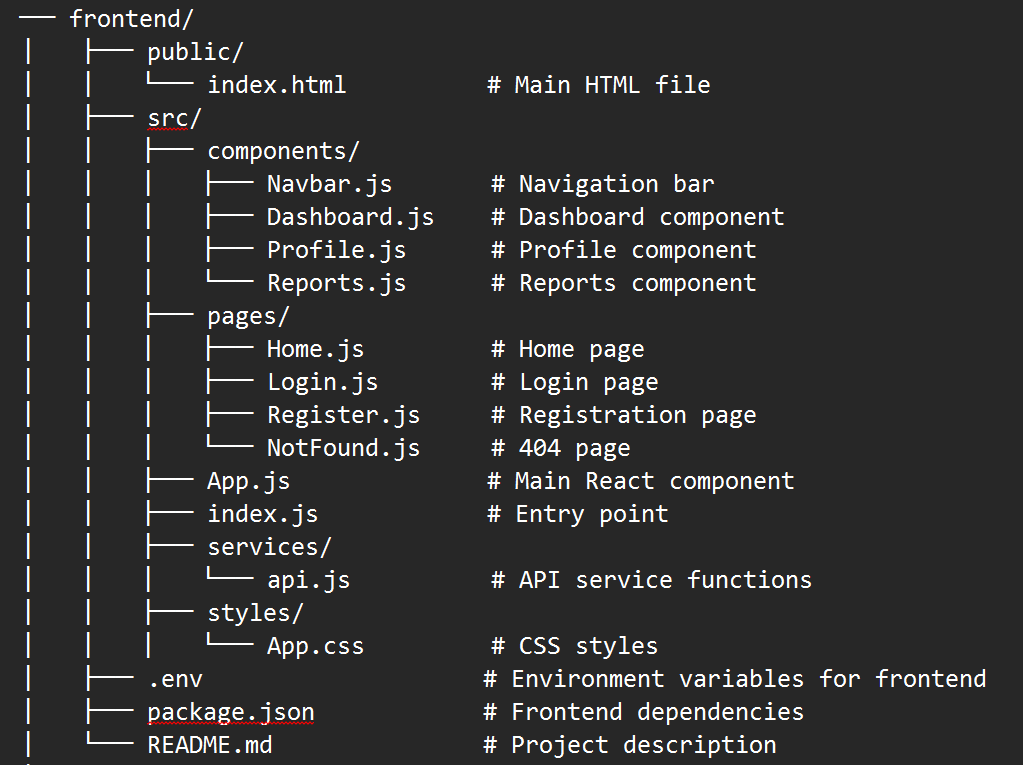
\includegraphics[width=0.7\textwidth]{images/frontend_file_structure.png}
    \caption{Frontend file structure}
    \label{fig:frontend file structure}
\end{figure}

\subsection{Frontend (React.js)}
\begin{itemize}
    \item \textbf{React.js:} Used for creating a dynamic, component-based user interface.
    \item \textbf{Material UI:} Provides pre-built UI components for a responsive and accessible interface.
    \item \textbf{Axios:} Handles API requests efficiently.
    \item \textbf{React Router:} Enables navigation between different sections of the application.
\end{itemize}


\subsection{Backend (Node.js and Express.js)}
\begin{itemize}
    \item \textbf{Express.js:} Facilitates the development of RESTful APIs.
    \item \textbf{MongoDB:} Stores user, NGO, company, and donation-related data in a structured format.
    \item \textbf{Mongoose:} Provides an Object Data Modeling (ODM) library for MongoDB.
    \item \textbf{JSON Web Tokens (JWT):} Ensures secure authentication and authorization.
    \item \textbf{Bcrypt.js:} Used for password hashing to enhance security.
\end{itemize}
\begin{figure}[h]
    \centering
    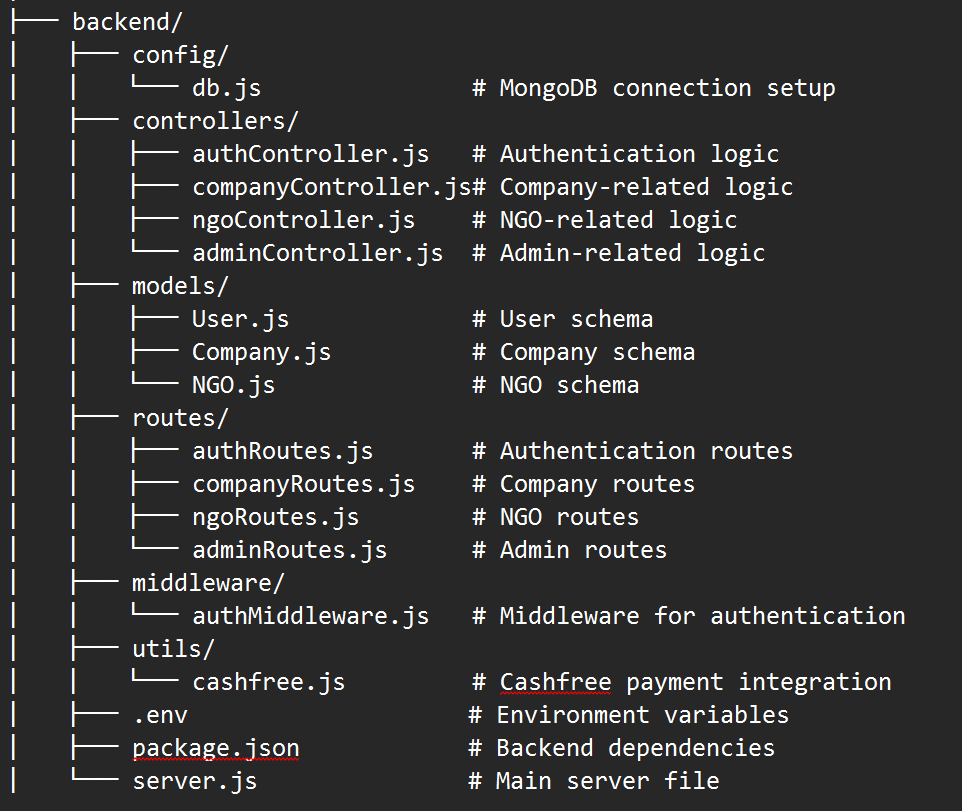
\includegraphics[width=0.7\textwidth]{images/backend_file_structure.png}
    \caption{Backend file structure}
    \label{fig:backend file structure}
\end{figure}

\subsection{Payment Gateway (Cashfree)}
\begin{itemize}
    \item Securely processes transactions and generates payment receipts.
    \item Ensures fraud detection and compliance with financial regulations.
\end{itemize}

\subsection{Deployment}
\begin{itemize}
    \item \textbf{Frontend Hosting:} Deployed using \textit{Vercel / Netlify}.
    \item \textbf{Backend Hosting:} Hosted on \textit{AWS EC2 / DigitalOcean}.
    \item \textbf{Database Hosting:} MongoDB Atlas for cloud-based NoSQL database management.
\end{itemize}

\section{System Modules and Implementation}
The platform consists of multiple modules, each implemented with specific functionalities:

\subsection{User Authentication}
\begin{itemize}
    \item \textbf{Signup/Login:} Implemented role-based authentication for \textbf{Admin, NGO, and Donor}.
    \item \textbf{JWT-based Authentication:} Each user receives a token upon login, ensuring secure access.
    \item \textbf{Password Hashing:} User passwords are stored securely using Bcrypt.
\end{itemize}
\begin{figure}[h]
    \centering
    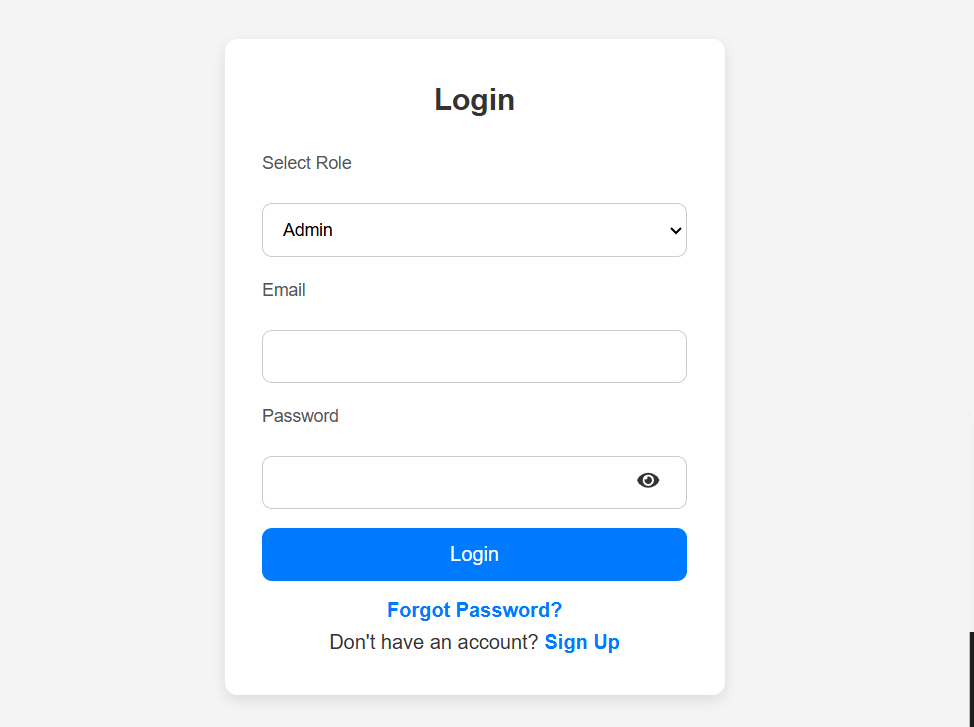
\includegraphics[width=0.7\textwidth]{images/login.png}
    \caption{Login Page}
    \label{fig: Login page}
\end{figure}

\subsection{NGO Management}
\begin{itemize}
    \item \textbf{NGO Registration:} Allows NGOs to register with details such as name, email, registered year, and address.
    \item \textbf{Profile Management:} NGOs can update their profiles and provide details about their activities.
    \item \textbf{Campaign Creation:} NGOs can create fundraising campaigns with images, descriptions, and funding goals.
\end{itemize}

\subsection{Campaign Management}
\begin{itemize}
    \item \textbf{Create Campaign:} NGOs can launch donation campaigns with goal amounts and deadlines.
    \item \textbf{View Campaigns:} Donors and companies can browse active campaigns.
    \item \textbf{Share Campaigns:} Generates a sharable campaign link for external donors.
\end{itemize}

\subsection{Donation Processing}
\begin{itemize}
    \item \textbf{Secure Transactions:} Cashfree Payment Gateway handles payment processing.
    \item \textbf{Donation Tracking:} Each donation is recorded in the system and linked to the donor and campaign.
    \item \textbf{Receipt Generation:} Generates digital receipts for donors after a successful donation.
\end{itemize}

\subsection{Admin Panel}
\begin{itemize}
    \item \textbf{Dashboard:} Displays reports on total donations, campaigns, and registered NGOs.
    \item \textbf{User Management:} Admin can approve, disable, or edit NGOs and campaigns.
    \item \textbf{Reports:} Generates detailed donation reports, including NGO performance.
\end{itemize}
\begin{figure}[h]
    \centering
    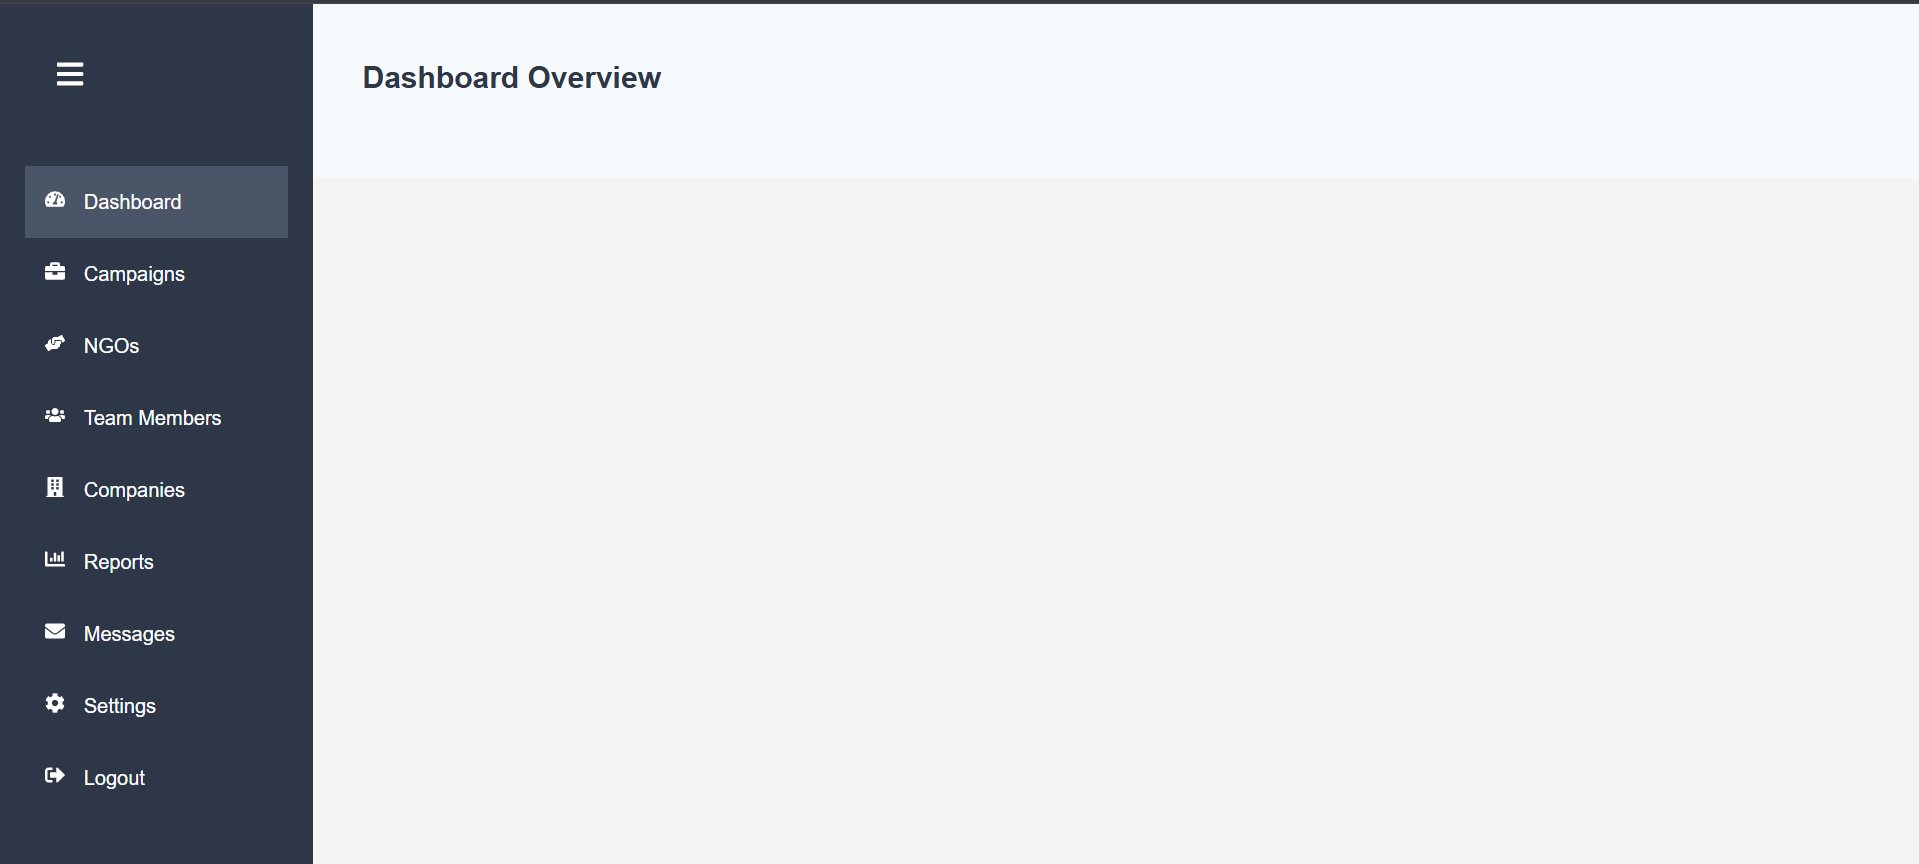
\includegraphics[width=0.7\textwidth]{images/admin_dashboard.png}
    \caption{Admin Dashboard}
    \label{fig: admin dashboard}
\end{figure}

\section{API Implementation}
\subsection{User Authentication API}
\begin{itemize}
    \item \textbf{POST /signup:} Registers a new user (Admin, NGO, or Donor).
    \item \textbf{POST /login:} Authenticates the user and returns a JWT token.
    \item \textbf{POST /change-password:} Allows users to update their password.
\end{itemize}
\begin{figure}[h]
    \centering
    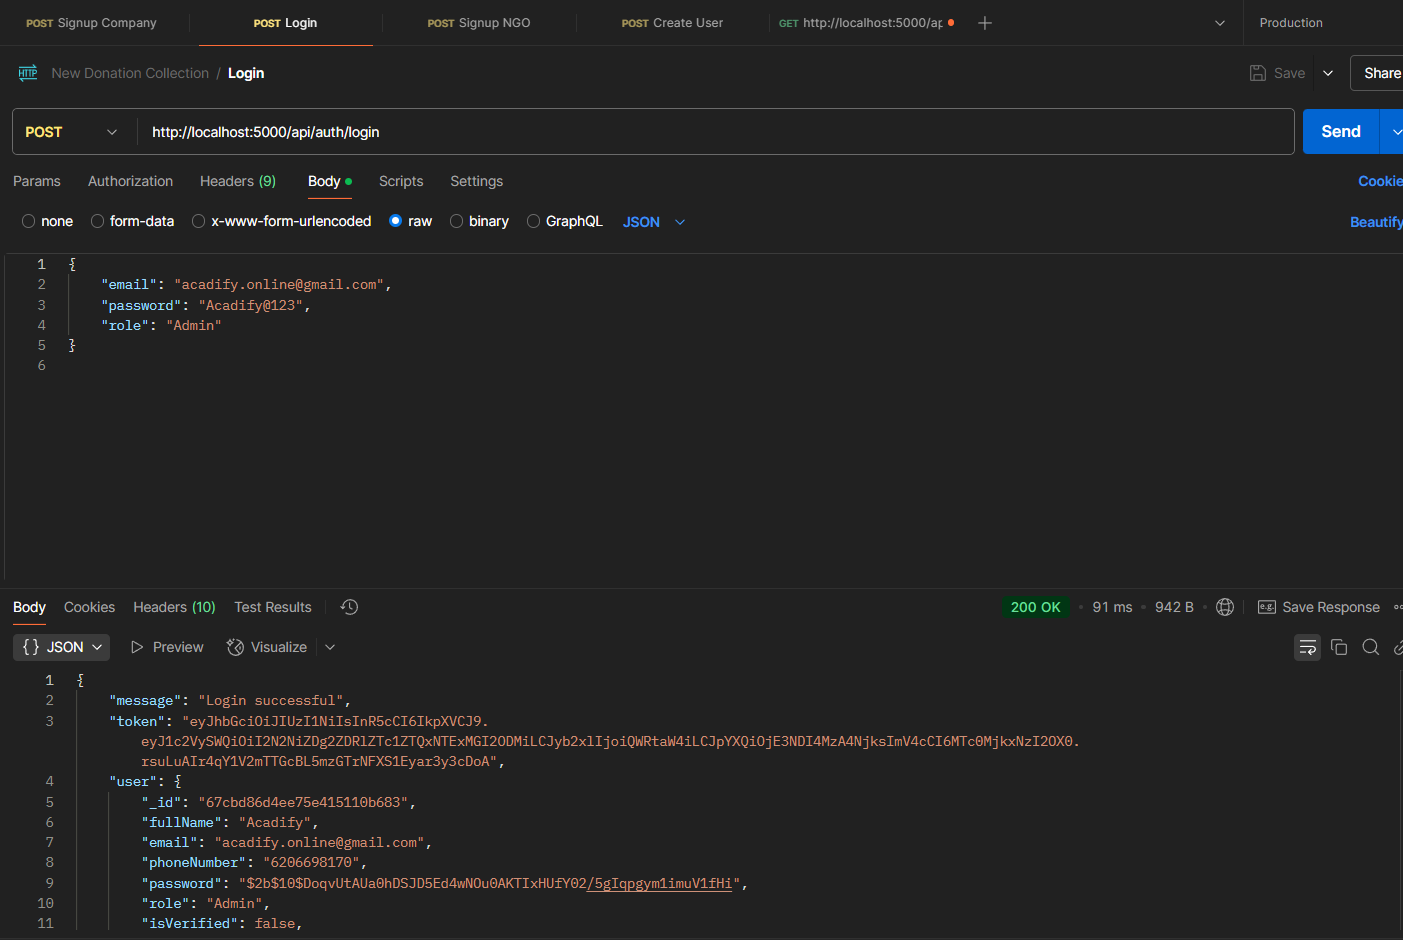
\includegraphics[width=0.7\textwidth]{images/User_Authentication_API.png}
    \caption{User Authentication API}
    \label{fig: User Authentication API}
\end{figure}

\subsection{NGO and Campaign APIs}
\begin{itemize}
    \item \textbf{GET /ngos:} Fetches all registered NGOs.
    \item \textbf{POST /create-campaign:} Creates a new fundraising campaign.
    \item \textbf{GET /campaigns:} Retrieves all active campaigns.
\end{itemize}
\begin{figure}[h]
    \centering
    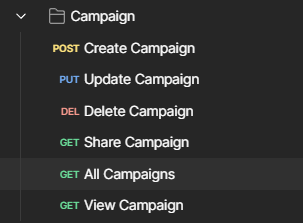
\includegraphics[width=0.5\textwidth]{images/Campaign.png}
    \caption{Campaign}
    \label{fig: Campaign}
\end{figure}

\subsection{Donation API}
\begin{itemize}
    \item \textbf{POST /donate:} Processes a donation using Cashfree.
    \item \textbf{GET /donations:} Retrieves all donations made by a specific donor.
    \item \textbf{GET /donation-receipt/:id:} Generates and provides the donation receipt.
\end{itemize}

\section{Testing and Debugging}
During implementation, various testing strategies were applied:

\subsection{Unit Testing}
\begin{itemize}
    \item Conducted using Jest and Mocha for individual API routes.
    \item Verified authentication, data validation, and payment processing functions.
\end{itemize}

\subsection{Integration Testing}
\begin{itemize}
    \item Ensured that frontend and backend components interact correctly.
    \item Validated end-to-end transaction processing using Postman.
\end{itemize}

\subsection{User Acceptance Testing (UAT)}
\begin{itemize}
    \item Conducted with real users (NGOs and donors) to gather feedback.
    \item UI enhancements were made based on user experience reports.
\end{itemize}

\section{Challenges and Solutions}
\subsection{Security Challenges}
\begin{itemize}
    \item Challenge: Ensuring secure transactions and user authentication.
    \item Solution: Implemented JWT authentication, password hashing, and HTTPS encryption.
\end{itemize}

\subsection{Scalability Issues}
\begin{itemize}
    \item Challenge: Handling a large number of donations and NGOs.
    \item Solution: Optimized database queries and used indexing in MongoDB.
\end{itemize}

\section{Deployment}
\subsection{Frontend Deployment}
\begin{itemize}
    \item Deployed using Vercel for continuous integration and seamless updates.
\end{itemize}

\subsection{Backend Deployment}
\begin{itemize}
    \item Hosted on AWS EC2 / DigitalOcean with auto-scaling configurations.
\end{itemize}

\subsection{Database Deployment}
\begin{itemize}
    \item MongoDB Atlas provides cloud-hosted NoSQL database services.
\end{itemize}
